\documentclass[11pt]{scrartcl}
\usepackage{color}
%\usepackage{enumitem}
%\setlist[itemize,2]{label=\textbullet}
\usepackage{geometry}
\geometry{a4paper, top=25mm, left=20mm, right=20mm, bottom=40mm, headsep=10mm, footskip=5mm}
\usepackage{ucs}
\usepackage[utf8x]{inputenc}
%\usepackage{german}
\usepackage{soul}
\usepackage{amsmath,amssymb,amstext}
\usepackage{graphicx}
\usepackage[automark]{scrpage2}
\usepackage{subcaption}
\usepackage{footnote}
\makesavenoteenv{tabular} %make footnotes in tables and tabulars appear
\makesavenoteenv{table}
%\usepackage{caption}
%\usepackage{subfigure}
%\usepackage{subfig}

\usepackage{algpseudocode,algorithm,algorithmicx}
\newcommand*\DNA{\textsc{dna}}

\newcommand*\Let[2]{\State #1 $\gets$ #2}
\algrenewcommand\algorithmicrequire{\textbf{Precondition:}}
\algrenewcommand\algorithmicensure{\textbf{Postcondition:}}

\usepackage[ngerman]{babel} 
\usepackage{xspace}
\usepackage{hyperref}
%\RequirePackage[ngerman=ngerman-x-latest]{hyphsubst}
\newcommand{\Gu}{\glqq{}}		%Gänsefüßchen unten
\newcommand{\Go}{\grqq\xspace} 
\newcommand{\red}{\textcolor{red}}
\newcommand{\ita}{\item[$\rightarrow$]}
\DeclareSymbolFont{matha}{OML}{txmi}{m}{it}% txfonts
\DeclareMathSymbol{\varv}{\mathord}{matha}{118}
\renewcommand*\labelitemii{-}
%\newcommand{\tightemize}{\vspace{-2mm}\begin{itemize}\setlength\itemsep{0em}}
\pagestyle{scrheadings}
\pagenumbering{arabic}	        %Gänsefüßchen oben
 \addtolength{\textheight}{25mm}
%\title{Lernende und Planende Roboter}
%\author{Sophie v. Schmettow}
%\date{\today{} in Karlsruhe}

\begin{document}

%----------------------------------------------------------------------------------------
%	TITLE PAGE
%----------------------------------------------------------------------------------------
\begin{titlepage}

\begin{center}


% Upper part of the page

\includegraphics[width=0.4\textwidth]{Logo_KIT.png}\\[1cm]    



\textsc{\Large Zusammenfassung}\\[0.5cm]


% Title
{ \huge \bfseries Mensch Maschine Interaktion}\\[0.4cm]
{ \large \bfseries Institut für Telematik -- Lehrstuhl für Pervasive Computing Systems}
\bigskip

% Author and supervisor

Sophie \textsc{v. Schmettow}\\
SoSe 16\\



\vfill

% Bottom of the page
{\large \today{} in Karlsruhe} 

\end{center}


\end{titlepage}

%----------------------------------------------------------------------------------------
%	ARTICLE CONTENTS
%----------------------------------------------------------------------------------------

\tableofcontents
\newpage

%----------------------------------------------------------------------------------------
%	UTILS
%----------------------------------------------------------------------------------------

%\begin{figure*}[ht]\centering % Using \begin{figure*} makes the figure take up the entire width of the page
%\includegraphics[width=\linewidth]{view}
%\caption{Wide Picture}
%\label{fig:view}
%\end{figure*}



%\begin{equation}
%\cos^3 \theta =\frac{1}{4}\cos\theta+\frac{3}{4}\cos 3\theta
%\label{eq:refname2}
%\end{equation}



%\begin{enumerate}[noitemsep] % [noitemsep] removes whitespace between the items for a compact look
%\item First item in a list
%\item Second item in a list
%\item Third item in a list
%\end{enumerate}



%\begin{figure}[ht]\centering
%\includegraphics[width=\linewidth]{results}
%\caption{In-text Picture}
%\label{fig:results}
%\end{figure}

%Reference to Figure \ref{fig:results}.


%\begin{table}[hbt]
%\caption{Table of Grades}
%\centering
%\begin{tabular}{llr}
%\toprule
%\multicolumn{2}{c}{Name} \\
%\cmidrule(r){1-2}
%First name & Last Name & Grade \\
%\midrule
%John & Doe & $7.5$ \\
%Richard & Miles & $2$ \\
%\bottomrule
%\end{tabular}
%\label{tab:label}
%\end{table}



%\begin{description}
%\item[Word] Definition
%\item[Concept] Explanation
%\item[Idea] Text
%\end{description}

%----------------------------------------------------------------------------------------
%	ARTICLE CONTENTS
%----------------------------------------------------------------------------------------

\section*{Disclaimer}
Dieses Dokument wurde im Rahmen des Master-Studiums
für das Modul \glqq Mensch-Maschine-Interaktion\grqq{} erstellt. Es stellt eine 
Zusammenfassung dar und dient zur Vorbereitung auf die
mündliche Prüfung. Neben den Materialien der Vorlesung
fließen auch weitere Quellen ein, um den behandelten Stoff
auszuarbeiten. Auf den Verweis von Quellen wird verzichtet,
da die Erstellung keinerlei wissenschaftlichen Zweck verfolgt
und nur für den privaten Gebrauch bestimmt ist.


%Lecture Content Overview (VL1, F24):
%1) Basics of Cognitive Science
%- Human Information Processing
%- Perception
%2) Formative Design and Evaluation of Human Computer Interaction (HCI)
%- Methods and Tools for Design
%3) Summative Evaluation of HCI
%- Basics of Human Studies and Statistics for Studies
%4) Best Practice in HCI
%- Concepts, Models, Guidelines, Methods

\section{Einführung} %(1. VL)
\subsection{Definitionen}
\begin{itemize}
	\item \textbf{Pervasive Computing}
	\begin{itemize}
		\item Pervasive Computing $\approx$ Ubiquitous Computing
		\item pervasive = \textit{alles durchdringend}
		\item IBM-Definition: \glqq Convenient access, through a new class of appliances, to relevant information with the ability to easily take action on it when and where you need\grqq
		\item Beispiel: Smartphones $\rightarrow$ relativ neue Technologie, daher viel höhrere Dynamik in der Entwicklung als beim Desktop. 
		\item Implizite Interaktionen: Gerät reagiert implizit auf User-Aktivität (insbesondere bei Smart Homes), jüngere lernen das besser (je älter man wird, desto mehr muss man anhand von Bezügen zu bereits Gelerntem/Metaphern lernen)
	\end{itemize}
	\item \textbf{Human Adopted Production}
	\begin{itemize}
		\item Comber and Maltby (1997) found that both overly simple and overly complex computing interfaces were low in usability 
		\item Wie kann man den User \glqq bei Laune halten\grqq ?\\
	 	$\rightarrow$ Die aktuell erfahrene Komplexität muss im Mittelmaß sein\\
	 	$\rightarrow$ Lernsysteme greifen per GSR Stress Level des Users ab und tunen dementsprechend das Lernsystem\\
	 	$\rightarrow$ kognitive Paramater sind sehr individuell
		\begin{figure}[h!]
			\centering
			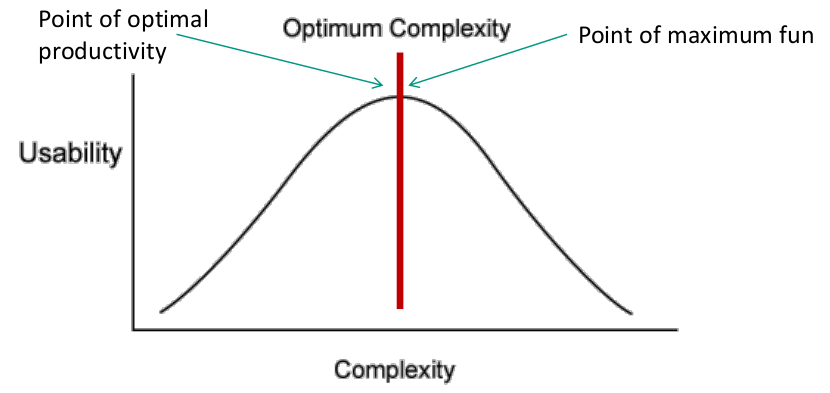
\includegraphics[width=.4\textwidth]{img/ch01_HAP.png}
			\caption{Human Adopted Production}
			\label{HAP}
		\end{figure} 
	\end{itemize}
	\item \textbf{Mensch-Maschine Interaktion}
	\begin{itemize}
		\item Important part of Pervasive Computing, e.g. Mobile Phone interfaces
		\item Pervasive Computing Technology produces now most/all innovative human machine interfaces, e.g. augmented reality glasses
	\end{itemize}
\end{itemize}
\subsection{Anwendungen}
\begin{itemize}
	\item Reprogramming Senses: Proxmity Helmet (mit Arduino) $\rightarrow$ wird nach einer Weile zum Gefühl, so kann man neue Sinne erschaffen
	\item Augmented Reality, Mobile Computing User Interface Software Design
	\item Wearable Thermography: detektiert Überbelastung bei Sport...
	\item Ubiquitous Sensing: Lobster House, Büro welches sich nach Sonne dreht, jeder Quadratmeter individuell klimatisierbar
\end{itemize}





\section{Human Information Processing (HIP)}

\section{Perception}

\section{Models and Concepts}

\section{Design Analysis}

\section{Interface and Interaction}

\section{Interaction Design}



\end{document}


%%% Local Variables:
%%% mode: latex
%%% TeX-master: t
%%% End: